\section{Dataset Statistics}
\label{sec:statistics}

\subsection{Overview}
\label{ssec:stats_overview}

Table~\ref{tab:dataset_overview} provides a high-level summary of \lucid{}. The
dataset is publicly released in three official splits: \textit{train} (8,993 scenarios,
70\%), \textit{validation} (1,927 scenarios, 15\%), and \textit{test} (1,927 scenarios,
15\%). The test split is held out and evaluated exclusively via an online evaluation
server to prevent overfitting to test labels.

\begin{table}[htbp]
  \centering
  \caption{\lucid{} dataset overview.}
  \label{tab:dataset_overview}
  \small
  \begin{tabular}{ll}
    \toprule
    \textbf{Property} & \textbf{Value} \\
    \midrule
    Total scenarios           & 12,847 \\
    Total driving duration    & $\sim$107 hours \\
    Total camera frames       & 2,312,460 \\
    Camera frame rate         & 10 FPS \\
    Camera resolution         & $1920 \times 1080$~px $\times$ 8 cameras \\
    LiDAR frame rate          & 20~Hz (top), 25~Hz (corner) \\
    Geographic coverage       & 6 cities, 3 continents \\
    Weather conditions        & 7 types \\
    Lighting conditions       & 4 types \\
    Total language annotations & 847,293 \\
    --- Causal QA pairs       & 312,456 \\
    --- Counterfactual QA pairs & 198,327 \\
    --- Planning instructions & 156,832 \\
    --- Scene descriptions    & 89,247 \\
    --- Risk assessments      & 90,431 \\
    Vocabulary size (unique tokens) & 84,732 \\
    Mean causal chain length (events) & 5.8 \\
    Mean counterfactual pairs per scenario & 15.4 \\
    Total annotators          & 234 \\
    Annotation person-hours   & $\sim$45,000 \\
    \midrule
    Train / Val / Test split  & 70\% / 15\% / 15\% \\
    \bottomrule
  \end{tabular}
\end{table}

\subsection{Scenario Distribution}
\label{ssec:stats_scenarios}

Figure~\ref{fig:distributions}(a) shows the distribution of scenarios across the five
scenario categories. Urban intersections form the largest category (29.9\%), reflecting
the high complexity and causal richness of intersection scenarios. Pedestrian-dense zones
(22.5\%) and long-tail edge cases (18.0\%) together account for over 40\% of the dataset,
ensuring robust coverage of safety-critical situations. The split is approximately balanced
to support learning across all scenario types without extreme class imbalance.

\subsection{Weather and Lighting Distribution}
\label{ssec:stats_weather}

\begin{figure}[htbp]
  \centering
  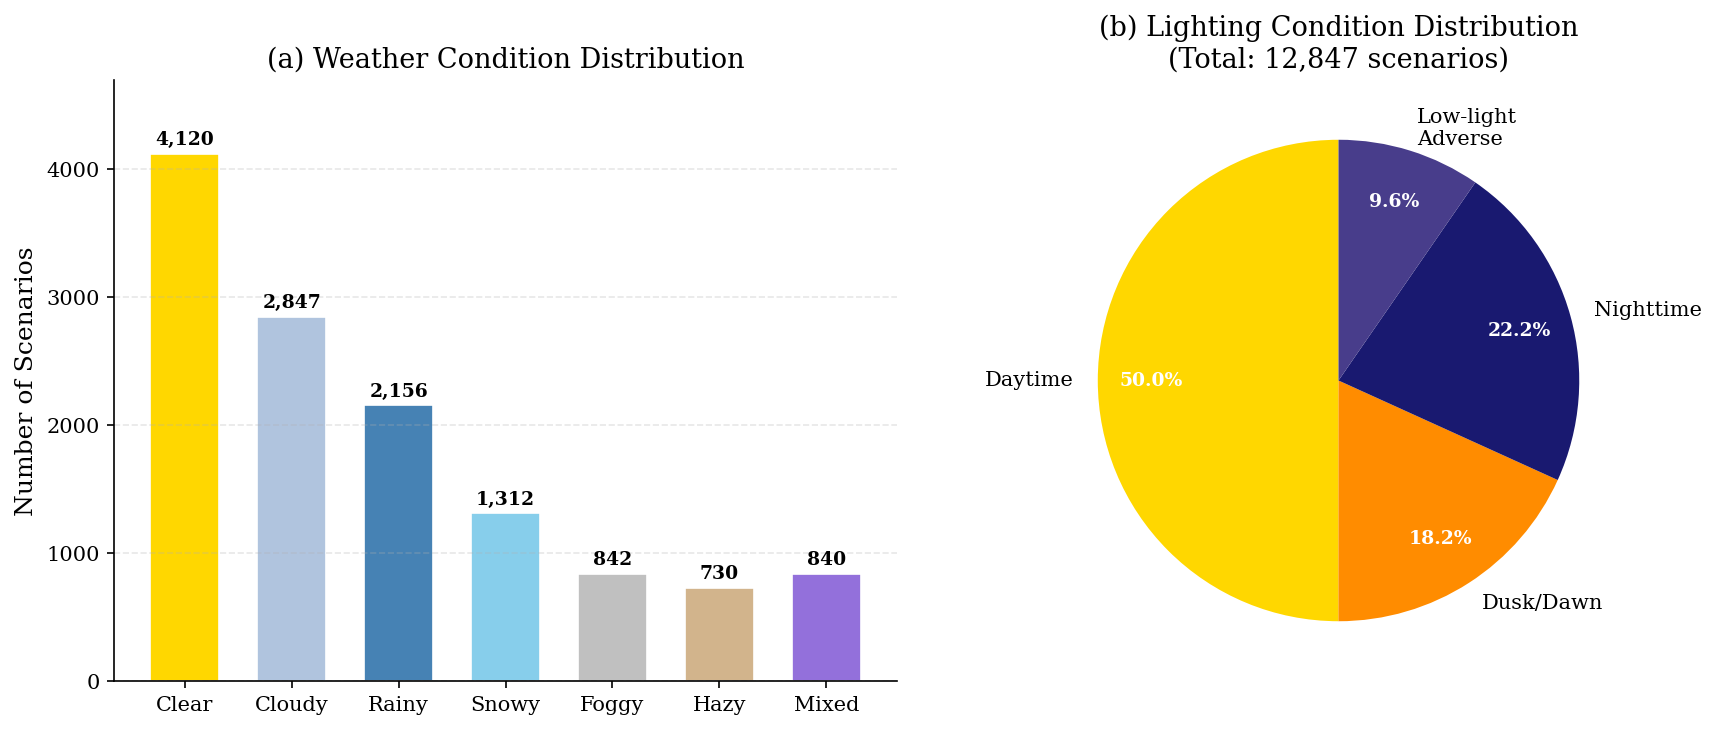
\includegraphics[width=\linewidth]{figures/weather_lighting.png}
  \caption{Left: distribution of the 12,847 scenarios across seven weather conditions.
  Right: distribution across four lighting conditions. The dataset provides substantial
  coverage of adverse conditions --- rainy (16.8\%), snowy (10.2\%), foggy (6.6\%), and
  night-time (22.2\%) scenarios constitute key additions beyond typical daylight-clear
  datasets.}
  \label{fig:weather_lighting}
\end{figure}

Figure~\ref{fig:weather_lighting} shows the weather and lighting distributions.
Clear weather scenarios represent 32.1\% of the dataset, while adverse conditions
(rain, snow, fog, haze, mixed) collectively account for 40.7\%. Nighttime scenarios
(22.2\%) and low-light adverse scenarios (9.6\%) provide critical coverage for
LLMs that must reason under degraded perception conditions. This distribution was
achieved through active scheduling of collection sessions during adverse weather
events and nighttime windows.

\subsection{Causal Chain Statistics}
\label{ssec:stats_causal}

The 312,456 causal QA pairs derive from 12,847 causal event graphs. The mean causal
chain length (number of event nodes in the CEG) is 5.8 (std 2.3, min 2, max 31).
Longer chains tend to occur in urban intersection and long-tail edge-case scenarios.
The most common causal root events include: \emph{unexpected pedestrian movement}
(18.3\%), \emph{vehicle lane change} (14.7\%), \emph{traffic signal state change}
(12.2\%), \emph{leading vehicle deceleration} (11.4\%), and \emph{road condition
change} (8.9\%).

\subsection{Counterfactual Statistics}
\label{ssec:stats_counterfactual}

The 198,327 counterfactual QA pairs average 15.4 per scenario. Three counterfactual
intervention types are represented: (1) \emph{agent-level interventions}
(``What if the pedestrian had not stepped off the curb?'') --- 52.3\% of pairs;
(2) \emph{environmental interventions} (``What if visibility had not been reduced by fog?'')
--- 28.7\% of pairs; and (3) \emph{ego-vehicle interventions} (``What if the ego
vehicle had been travelling at 70 km/h rather than 50 km/h?'') --- 19.0\% of pairs.

\subsection{Annotation Length and Vocabulary}
\label{ssec:stats_vocab}

The mean annotation length is 50.1 words per annotation across all types. Causal
QA answers are the longest (mean 58.7 words), as they must articulate multi-step
causal chains. The dataset vocabulary contains 84,732 unique tokens, significantly
richer than NuScenes-QA (template-derived, limited vocabulary) and comparable to
DriveLM. Annotations were authored in British English following a style guide to
maximise linguistic consistency.
